% !TeX TXS-program:compile = txs:///pdflatex/[--shell-escape]

\documentclass[11pt, letterpaper]{article}

\usepackage{minted}
\usepackage[utf8]{inputenc}
\usepackage[T1]{fontenc}
\usepackage{lmodern}
\usepackage{graphicx}
\usepackage{longtable}
\usepackage{wrapfig}
\usepackage{rotating}
\usepackage{amsmath}
\usepackage{textcomp}
\usepackage{amssymb}
\usepackage{hyperref}
\usepackage[round]{natbib}
\usepackage{subcaption}


\title{\bfseries Tarea}
\author{Ángel García Báez}
\date{\today}
\setcounter{tocdepth}{3} 

\begin{document}
	
	% Página de presentación
	\begin{titlepage}
		\centering
		
\includegraphics[width=0.2\textwidth]{logo.png}\par
		\vspace{1cm}
		{\LARGE \bfseries Universidad Veracruzana \par}
		\vspace{1cm}
		{\Large Maestría en Inteligencia Artificial\par}
		\vspace{3cm}
		{\LARGE \bfseries Visión por Computadora \par}
		\vspace{1cm}
		{\Large \bfseries Tarea 4. Implementación del operador de Sobel para detección de bordes en Julia y Matlab. \par}
		\vfill
		{\Large \textit{Ángel García Báez}\par}
		\vspace{1cm}
		{\Large Profesor: Dr. Héctor Acosta Mesa\par}
		\vfill
		{\Large \today \par}
	\end{titlepage}
	
	% Página exclusiva para la tabla de contenidos
	\newpage
	\tableofcontents
	\newpage
	
% Sección para el problema 1
\section{Objetivo de la práctica}
	
Se tiene la siguiente imagen en escala de grises:


\begin{figure}[h!]
	\centering
	\begin{minipage}{0.45\textwidth}
		\centering
		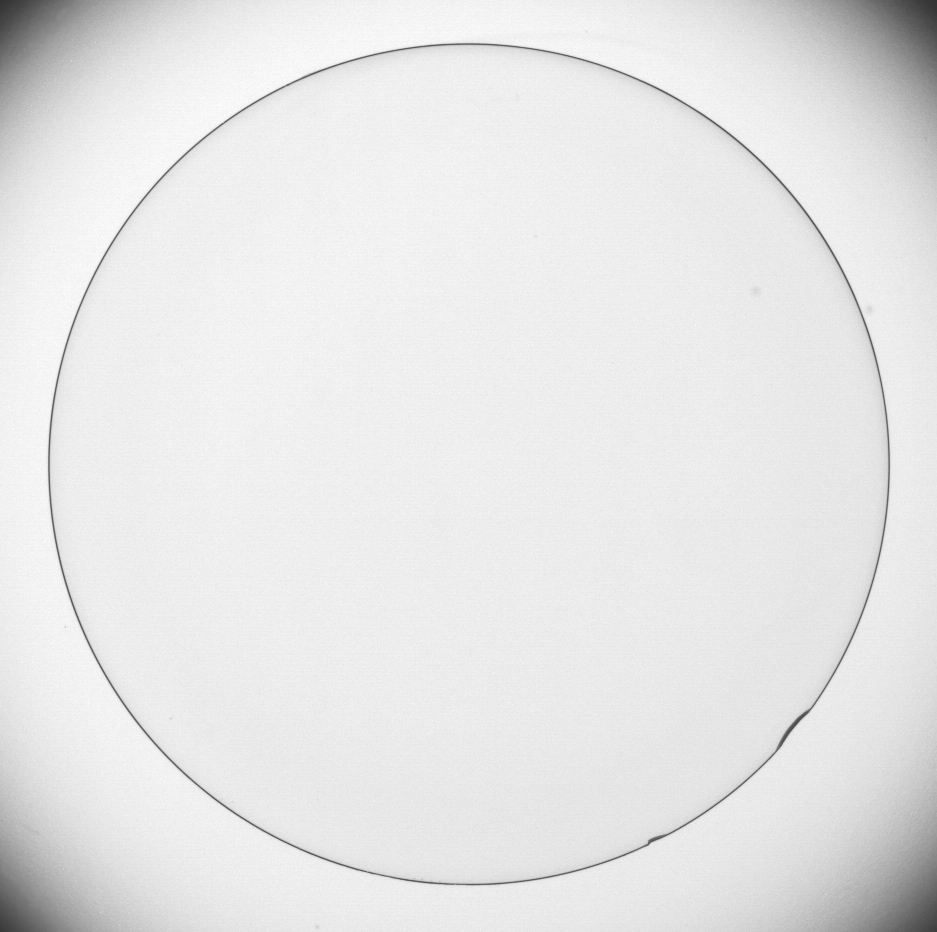
\includegraphics[width=\textwidth]{IMG/Fig3.45(a).jpg}
		\caption{Figura 3.45(a). Extraída del libro Digital Image Processing}
		\label{fig:f1}
	\end{minipage}\hfill
\end{figure}

El objetivo de la presente practica es implementar un algoritmo que aplique el operador de Sobel sobre la imagen para la correcta detección de bordes en la imagen.

Para ello, se pide que:

\begin{enumerate}
	\item Escribir un programa que haga el de los vectores gradientes usando el operador de Sobel sobre la figura 3.45.
	\item Motrar el resultado de del computo sobre $G_x$, $G_y$, $\nabla f$ y $\Theta$.
	\item  Mostrar los vectores como un flujo óptico de flechas perpendiculares al eje usando el comando de matlab $quiver(Gx,Gy)$.
	
	\item  Explique brevemente los resultados.
	
\end{enumerate}
	
	\newpage
	
	\section{Metodología}
	
	Para la correcta implementación del operador de Sobel es necesario definirlo en sus componentes más básicas, por lo que se recurrió al uso de las definiciones que vienen \cite{gonzalez2018digital}:
	
	El gradiente (primera derivada) de la una imagen, puede ser visto como una derivada bidimensional que tiene la siguiente forma:
	
	$$\nabla f \equiv \text{grad}(f) = \begin{bmatrix} g_x \\ g_y \end{bmatrix} = \begin{bmatrix} \frac{\partial f}{\partial x} \\ \frac{\partial f}{\partial y} \end{bmatrix}$$
	
	Se observa que para la construcción del gradiente $\nabla f$ se necesitan obtener los correspondientes $g_x$ y $g_y$ que corresponden a las derivadas parciales en $x$ y en $y$.
	
	Dado que los pixeles en una imagen no siguen el comportamiento de una función continua como tal, bajo ciertos arreglos y simplificaciones de muestreos locales, se puede construir un operador que calcula la derivada localmente mediante una mascara de 3x3 para la región que esta siendo muestreada bajo la siguiente estructura:
	
	$$
	\begin{bmatrix}
		z_1 & z_2 & z_3 \\
		z_4 & z_5 & z_6 \\
		z_7 & z_8 & z_9
	\end{bmatrix}
	$$
	
	Haciendo dichas simplificaciones, es posible obtener la derivada parcial en $x$ como sigue:
	
	$$g_x = \frac{\partial f}{\partial x} = (z_7 + 2z_8 + z_9) - (z_1 + 2z_2 + z_3)$$	
	
	Al visualizar los coeficientes como matriz, salta a la vista el objetivo el filtro, detectar los cambios en la derivada en la componente $x$:
	
	$$
	\begin{bmatrix}
		-1 & -2 & -1 \\
		0 & 0 & 0 \\
		1 & 2 & 1
	\end{bmatrix}
	$$
	
	
	Por otro lado, se tiene la correspondiente operación para el calculo de la derivada parcial en $y$ como sigue:	
	
	$$g_y = \frac{\partial f}{\partial y} = (z_3 + 2z_6 + z_9) - (z_1 + 2z_4 + z_7)$$

	\newpage
	
	Al visualizar los coeficientes como matriz, salta a la vista el objetivo el filtro, detectar los cambios en la derivada en la componente $y$:
	
	$$
	\begin{bmatrix}
		-1 & 0 & 1 \\
		-2 & 0 & 2 \\
		-1 & 0 & 1
	\end{bmatrix}
	$$
	
	Una vez que se cuentan con los elementos primarios se puede proceder con la construcción del gradiente. Cabe mencionar que el gradiente como tal, lo que hace es señalar la dirección de mayor cambio en la función en el punto $(x,y)$, por lo que se utiliza la norma del vector gradiente para conocer su norma.
	
	$$M(x, y) = ||\nabla f|| = \text{mag}(\nabla f) = \sqrt{G_x^2 + G_y^2}$$
	
	Finalmente, para calcular el angulo que se forma entre los vectores de las derivadas parciales $G_x$ y $G_y$ se utilizo la tangente inversa entre los vectores como se explica en \cite{perez2018procesamiento}:
	
	$$\theta(G_x,G_y) = \arctan(G_x,G_y )$$
	
	Se realizo la implementación en Julia por su simpleza y velocidad en el procesamiento de operaciones con matrices así como con matlab para el uso de la función quiver().
	
	Cabe mencionar que para el caso del procesamiento de las imagenes como matrices en Julia, fue necesario aplicar una normalización a los valores producidos por el operador de Sobel para que se encuentre en un rango entre 0 y 1. Dicha normalización para el caso de los resultados obtenidos para $G_x$, $G_y$ y $M(x,y)$ viene dada por:
	
	$$nomalizacion(M) = \frac{M-min(M)}{max(M)-min(M)}$$
	
	Donde $M$ es la matriz de valores resultantes para los 3 casos.
	
	Para el caso del angulo $\theta$ se aplico la normalización de forma distinta debido a que los valores  del angulo que devuelve Julia están dados en radianes:
	
	$$normalizacion(\theta) = \frac{\theta + \pi}{2 \pi}$$
	
	Por ultimo, se hizo uso de a función ya implementada en matlab $quiver()$ con las matrices de $G_x$ y $G_y$	obtenidas del proceso de aplicar el operador de Sobel.
	
\newpage
	
\section{Resultados}

A continuación se muestran los resultados obtenidos por la implementación en Julia y en matlab

\subsection{Resultados para Gx}

\begin{figure}[h]
	
	\begin{minipage}{0.48\textwidth} % Ajustamos el ancho para dejar un pequeño espacio entre las imágenes
		\centering
		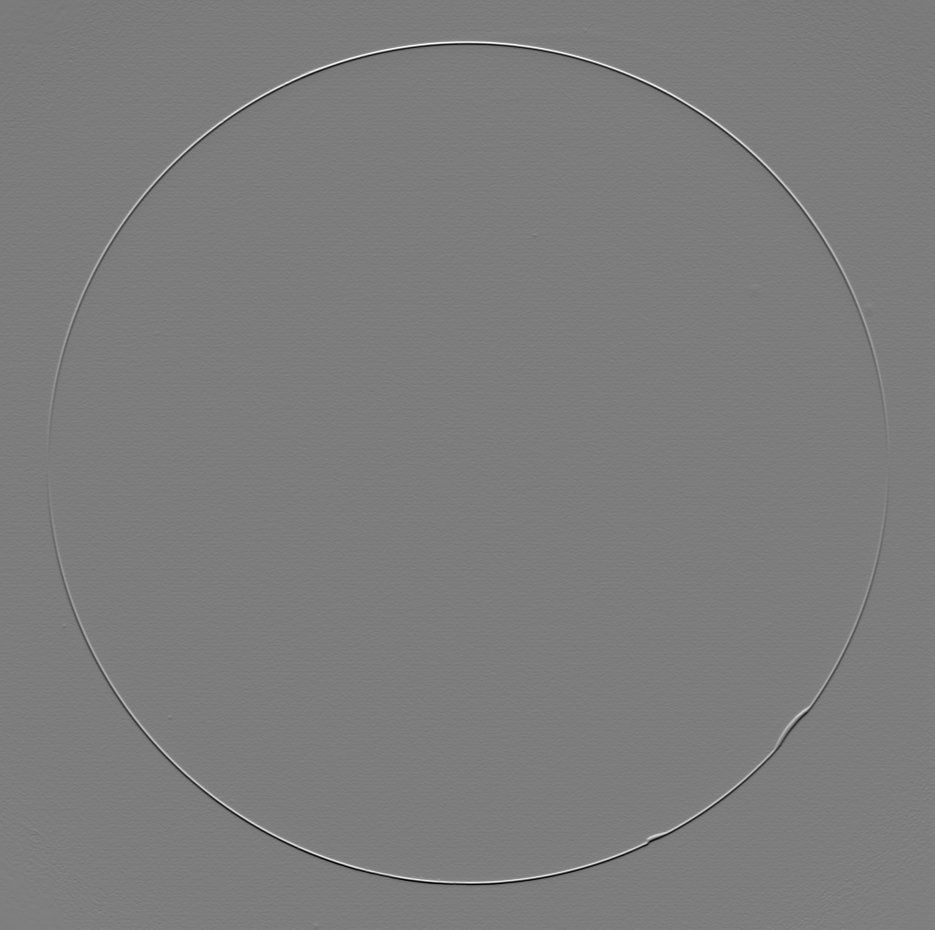
\includegraphics[width=\textwidth]{IMG/q21.png} % Ajusta la ruta y el nombre del archivo
		\caption{Gx en Julia.}
		\label{fig:img2}
	\end{minipage}\hfill % \hfill para separar las imágenes horizontalmente
	\begin{minipage}{0.48\textwidth} % Ajustamos el ancho para dejar un pequeño espacio entre las imágenes
		\centering
		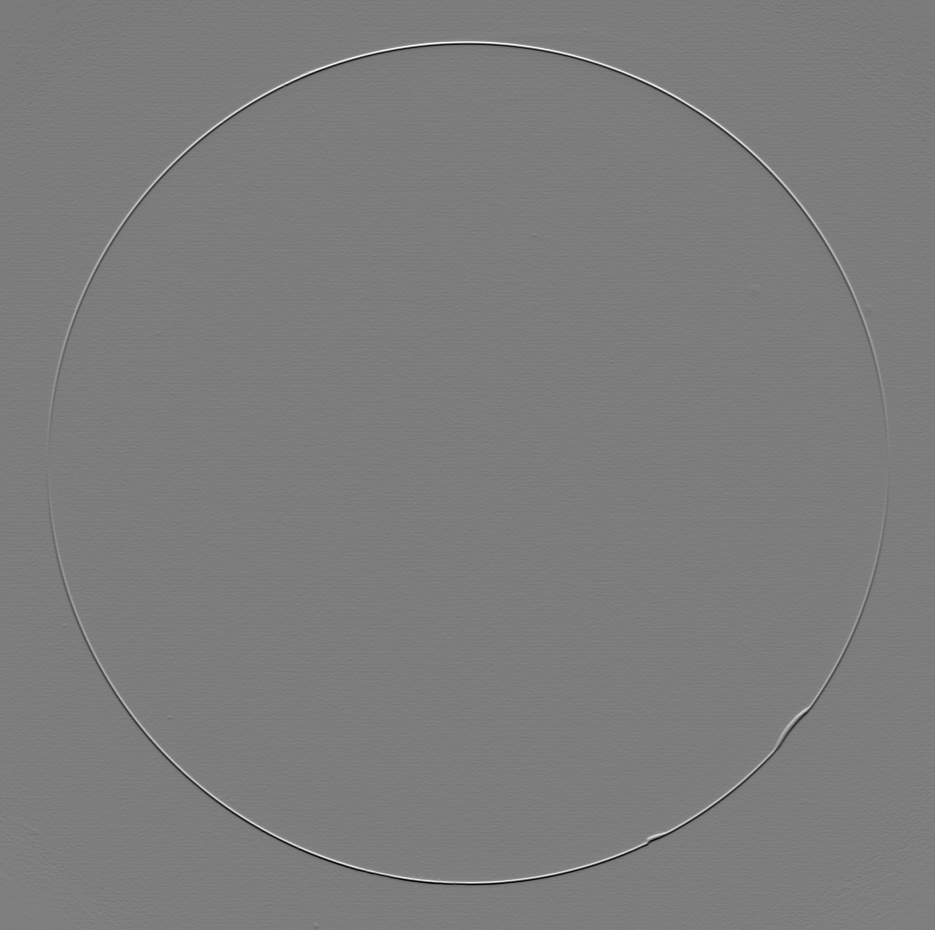
\includegraphics[width=\textwidth]{IMG/q2.png} % Ajusta la ruta y el nombre del archivo
		\caption{Gx en Matlab.}
		\label{fig:img3}
	\end{minipage}
	
	\caption{Comparación en Gx.}
	\label{fig:comparacion gx}
\end{figure}		

Se observa como ambos filtros logran detectar con mayor precisión los bordes que se generan en la curvatura del circulo que están en los extremos superiores e inferiores, dejando con una menor intensidad de detección la curvatura de los laterales y mostrando que el circulo presenta una pequeña deformidad en la parte inferior derecha.

Los resultados obtenidos entre ambas implementaciones son prácticamente el mismo.

\newpage

\subsection{Resultados para Gy}

\begin{figure}[h]
	
	\begin{minipage}{0.48\textwidth} % Ajustamos el ancho para dejar un pequeño espacio entre las imágenes
		\centering
		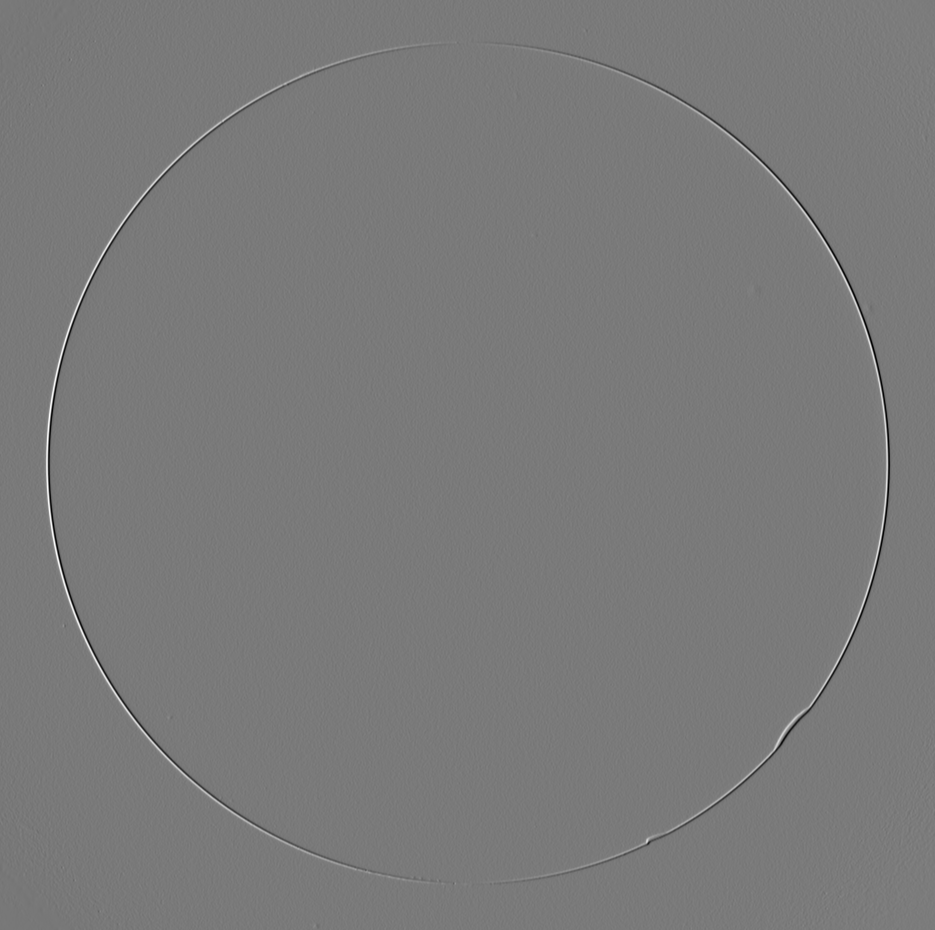
\includegraphics[width=\textwidth]{IMG/q11.png} % Ajusta la ruta y el nombre del archivo
		\caption{Gy en Julia.}
		\label{fig:img4}
	\end{minipage}\hfill % \hfill para separar las imágenes horizontalmente
	\begin{minipage}{0.48\textwidth} % Ajustamos el ancho para dejar un pequeño espacio entre las imágenes
		\centering
		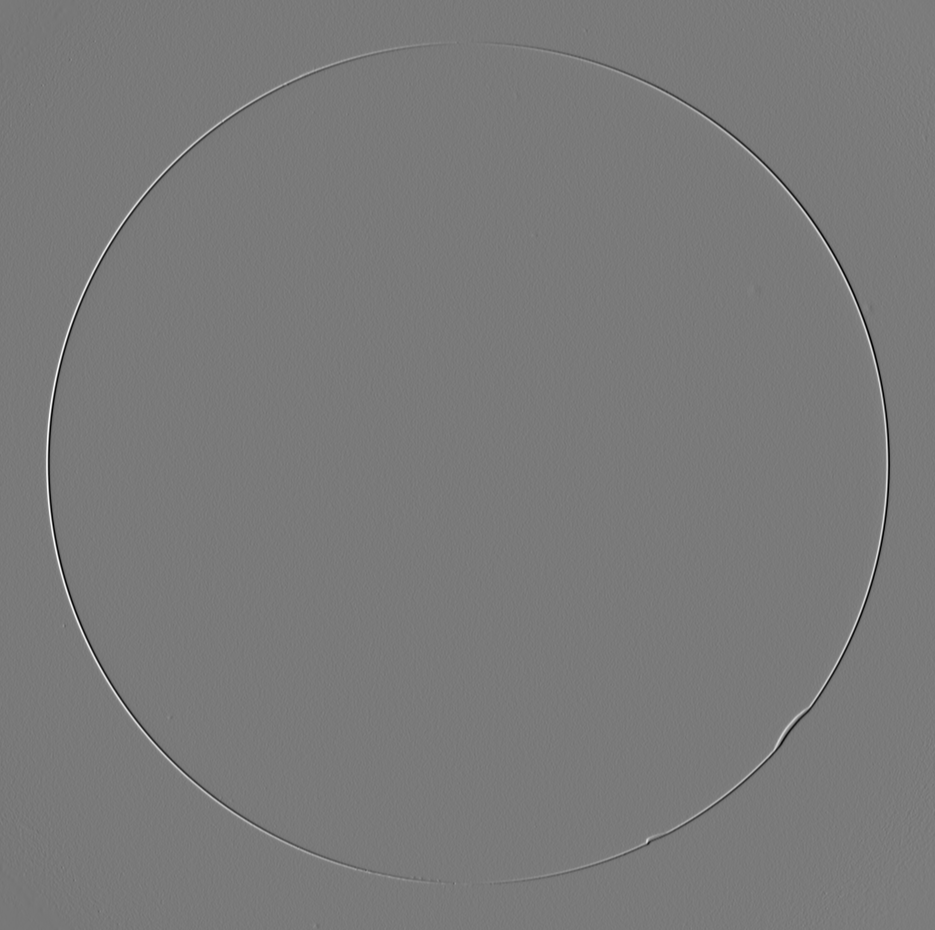
\includegraphics[width=\textwidth]{IMG/q1.png} % Ajusta la ruta y el nombre del archivo
		\caption{Gx en Matlab.}
		\label{fig:img5}
	\end{minipage}
	
	\caption{Comparación en Gy.}
	\label{fig:comparacion en gy}
\end{figure}		

Se observa como ambos filtros detectan mejor la curvatura de los laterales del circulo, dándole menos intensidad a la curvatura superior e inferior.

Los resultados obtenidos entre ambas implementaciones son prácticamente el mismo.

\newpage

\subsection{Resultados para el gradiente G}

\begin{figure}[h]
	
	\begin{minipage}{0.48\textwidth} % Ajustamos el ancho para dejar un pequeño espacio entre las imágenes
		\centering
		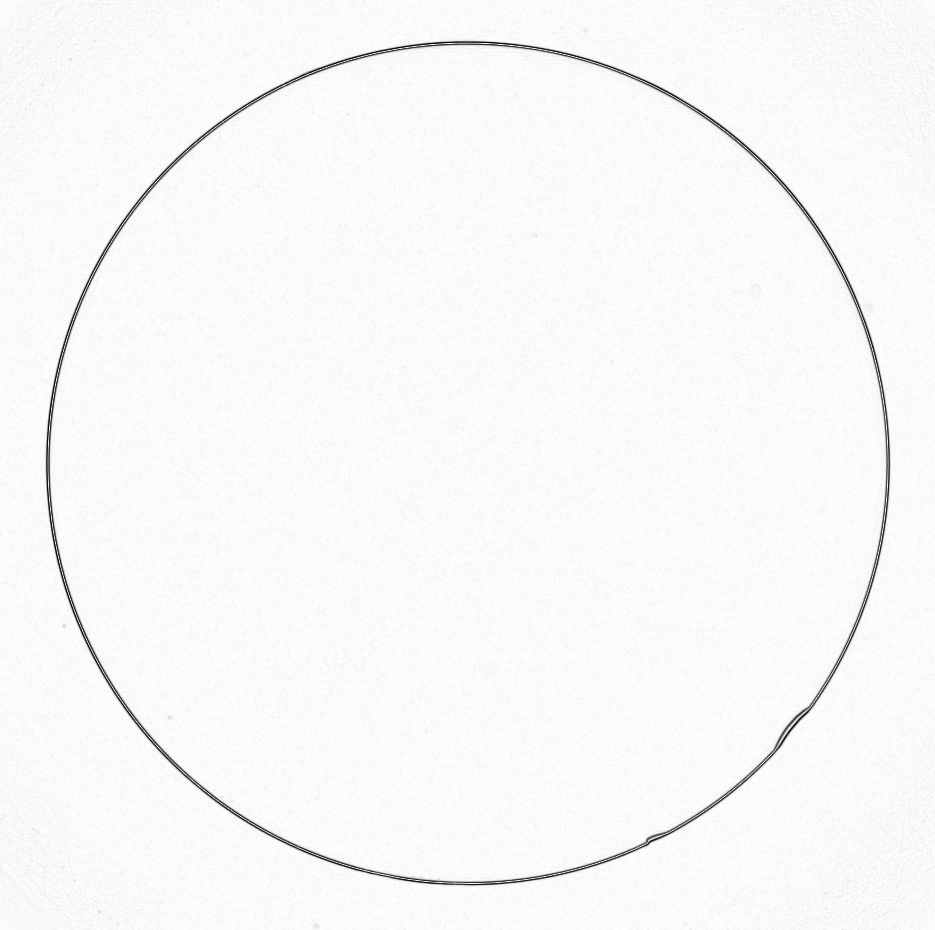
\includegraphics[width=\textwidth]{IMG/q31.png} % Ajusta la ruta y el nombre del archivo
		\caption{Gradiente en Julia.}
		\label{fig:img6}
	\end{minipage}\hfill % \hfill para separar las imágenes horizontalmente
	\begin{minipage}{0.48\textwidth} % Ajustamos el ancho para dejar un pequeño espacio entre las imágenes
		\centering
		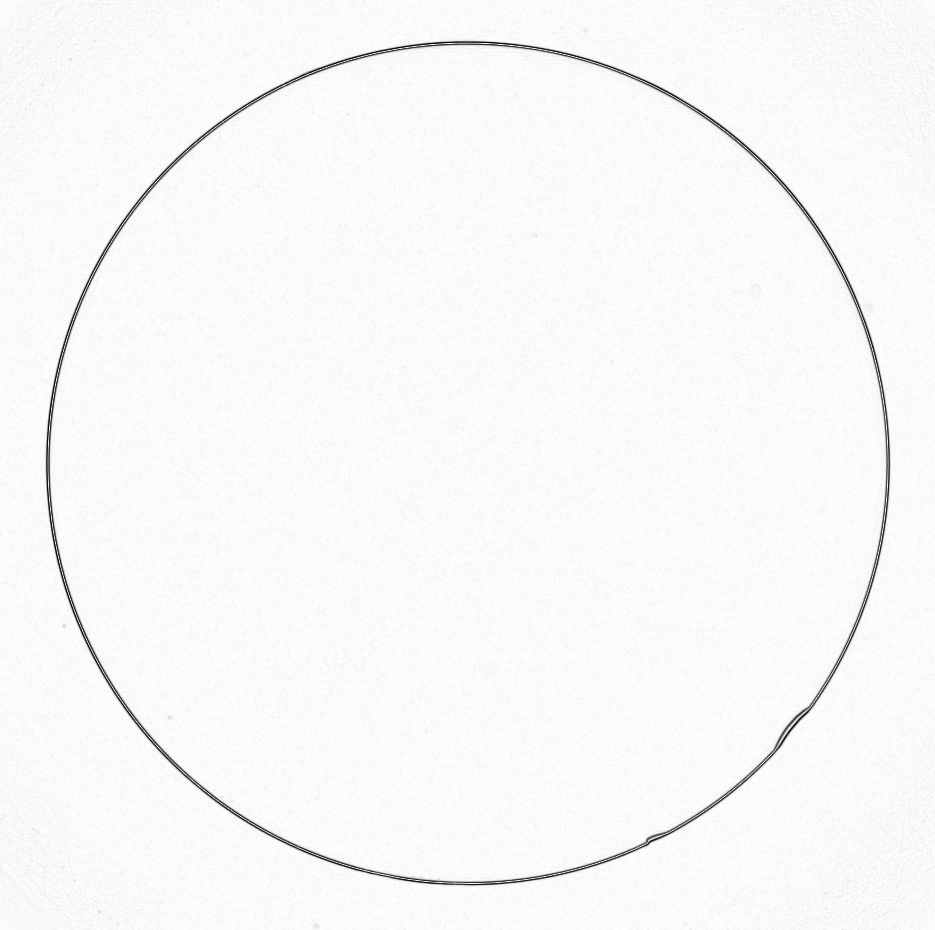
\includegraphics[width=\textwidth]{IMG/q3.png} % Ajusta la ruta y el nombre del archivo
		\caption{Gradiente en Matlab.}
		\label{fig:img7}
	\end{minipage}
	
	\caption{Comparación en G.}
	\label{fig:comparacion en G}
\end{figure}		

Lo primero que salta a la vista es como al combinar la información obtenida de $G_x$ y de $G_y$ para el gradiente de la imagen, la imagen mejora bastante al punto que resalta unicamente lo que detecta como borde, que en ambos casos es la completitud de la curvatura del circulo, eliminando a su paso todo aquello que no es borde según el operador.

\newpage

\subsection{Resultados para el angulo del gradiente}

\begin{figure}[h]	
	\begin{minipage}{0.48\textwidth} % Ajustamos el ancho para dejar un pequeño espacio entre las imágenes
		\centering
		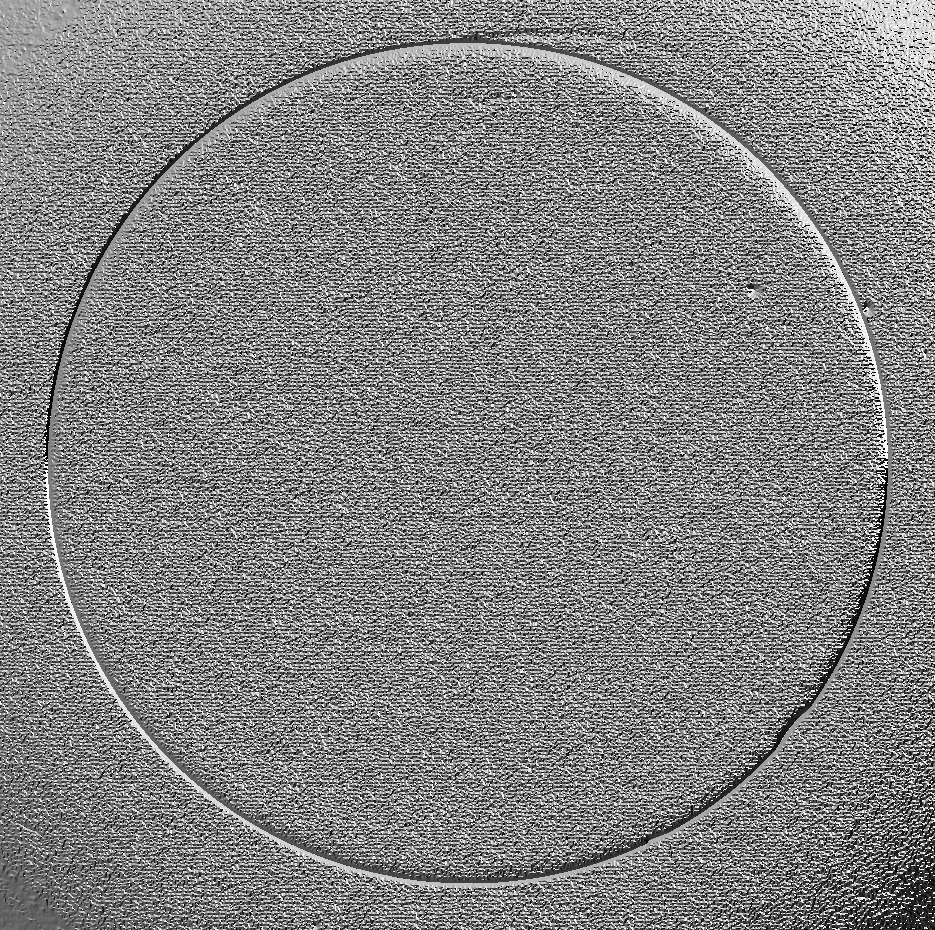
\includegraphics[width=\textwidth]{IMG/q41.png} % Ajusta la ruta y el nombre del archivo
		\caption{Angulo del gradiente en Julia.}
		\label{fig:img8}
	\end{minipage}\hfill % \hfill para separar las imágenes horizontalmente
	\begin{minipage}{0.48\textwidth} % Ajustamos el ancho para dejar un pequeño espacio entre las imágenes
		\centering
		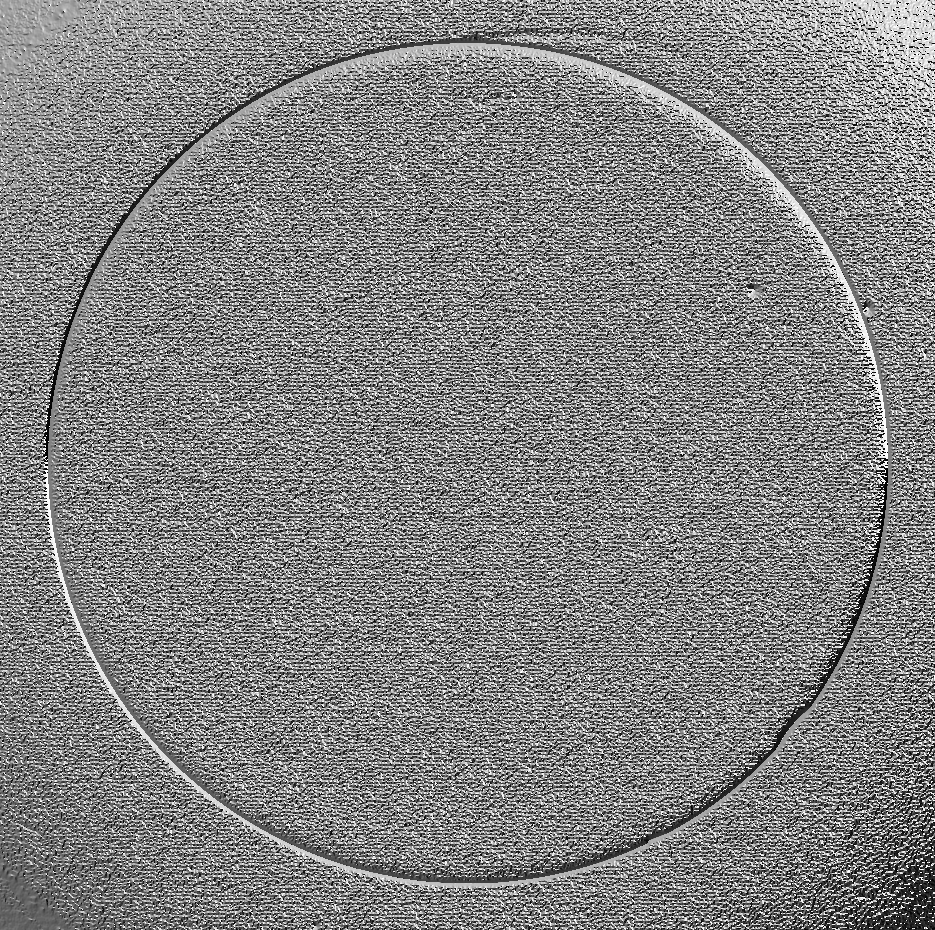
\includegraphics[width=\textwidth]{IMG/q4.png} % Ajusta la ruta y el nombre del archivo
		\caption{Angulo del gradiente en Matlab.}
		\label{fig:img9}
	\end{minipage}
	
	\caption{Comparación del Angulo del gradiente.}
	\label{fig:comparacion en Gradiente}
\end{figure}		

Se observa como la representación del angulo genera una imagen con lo que pareciera ser algún patrón de textura como si fuera tela estirada o papel aluminio doblado en donde resalta principalmente los bordes de la figura.

El resultado de graficar el angulo de los gradientes $Gx$ y $Gy$ es prácticamente el mismo en ambos casos.

\newpage

\subsection{Resultados de la función quiver}

\begin{figure}[h]
	\centering
	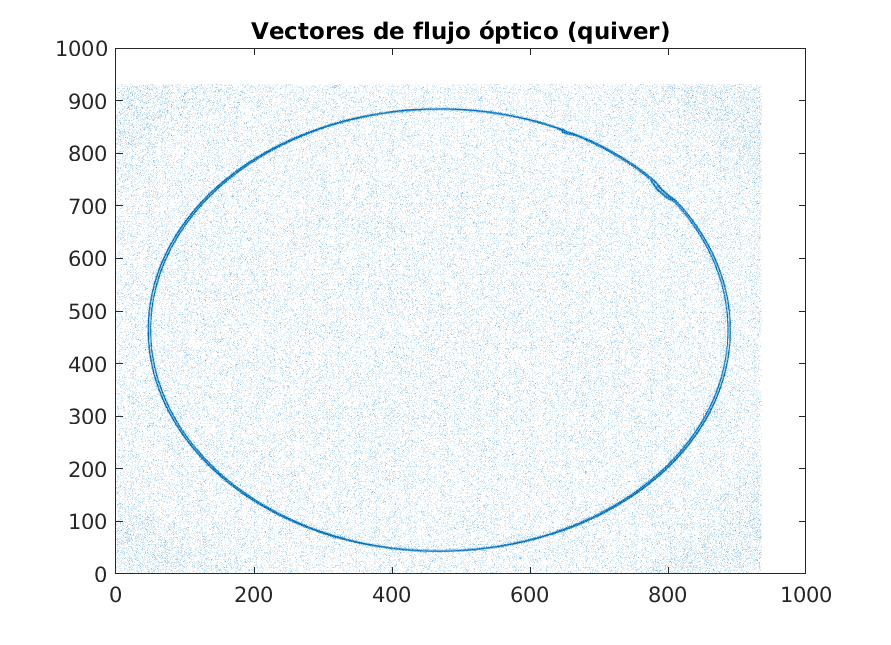
\includegraphics[width=\textwidth]{IMG/quiver.png} % Ajusta la ruta y el nombre del archivo
	\caption{Resultado de quiver sobre la imagen.}
	\label{fig:img10}
	\vspace{0.5cm} % Espacio vertical adicional entre las imágenes y la siguiente figura
	\label{fig:Quiver}
\end{figure}

El resultado de aplicar la función quiver en matlab da como resultado el mapeo de los bordes de la imagen con su representación como vectores (flechas). Salta a la vista que pese a que no se observan directamente los vectores, estos se encuentran acomodados alrededor del borde del circulo, formando a su vez el contorno de la figura.


\newpage
	
\section{Conclusiones}
	
Tras la implementación del algoritmo en ambos lenguajes de programación, se observo como no difieren prácticamente en nada los resultados de las implementaciones entre ambos lenguajes, esto se debe a que en esencia, están computando lo mismo ambos lenguajes. \\

Por otro lado, los resultados obtenidos por el operador de sobel resultan impresionantes debido a la precisión con la que logra extraer el borde de la imagen y eliminar todo lo que no representa un borde para el operador. \\

Finalmente, cabe mencionar que ya sea que se haga en un lenguaje u otro, es necesario tomar en cuenta la forma en que se hacen los cálculos internamente de las convolusiones, debido a que a medida que se pueda procesar una gran serie de imágenes o de altas resoluciones, la cantidad de operaciones que debe realizar el algoritmo aumenta rápidamente por lo que implicaría un mayor coste de tiempo y recurso computacional.

\newpage

	
\section{Referencias}  % Sección numerada de referencias
\bibliographystyle{apalike}  % Estilo de citas (puedes cambiarlo)
\bibliography{Biblio}        % Nombre del archivo BibTeX (sin extensión)

\newpage
	
\section{Anexos}	
\subsection{Implementación de la ecualización por histograma}
\begin{minted}[linenos,firstnumber=1]{julia}
#### Paquetes necesarios ####
using Plots
using Images
using StatsBase

# Función del gradiente de SOBEL #
function imsobel(img_ruta::String)
	# Cargar la imagen
	img = load(img_ruta)
	# Convertir la imagen a escala de grises y multiplicar por 255
	img1 = Gray.(img) .* 255
	# Generar la matriz que detecta en Gx
	gxk = [-1 0 1; -2 0 2; -1 0 1]
	# Generar la matriz que detecta en Gy
	gyk = gxk' # Usamos la transpuesta de gxk
	# Obtener las dimensiones de la imagen y el kernel
	imdim = size(img1)
	kerdim = size(gxk)
	# Calcular las dimensiones de la imagen resultante
	rf = imdim[1] - kerdim[1] + 1
	rc = imdim[2] - kerdim[2] + 1
	# Crear un array para guardar los resultados
	resultado = zeros(rf, rc, 4)
	# Aplicar la convolución
	for i in 1:rf
		for j in 1:rc
			# Extraer una submatriz de nxn de la imagen
			subim = img1[i:i+kerdim[1]-1, j:j+kerdim[2]-1]
			
			# Aplicar la convolución sobre GX
			resultado[i, j, 1] = sum(subim .* gxk)
			
			# Aplicar la convolución sobre GY
			resultado[i, j, 2] = sum(subim .* gyk)
			
			# Calcular el operador de Sobel
			sobel = sqrt(resultado[i, j, 1]^2 + resultado[i, j, 2]^2)
			
			# Guardar el valor del gradiente
			resultado[i, j, 3] = sobel
		end
	end
	#### Reportar las salidas ####
	# Reportar Gx
	rgx = resultado[:, :, 1]
	# Estandarizar
	minr = minimum(rgx)
	maxr = maximum(rgx)
	p1 = (rgx .- minr) ./ (maxr - minr)
	q1 = 1 .- p1
	# Reportar Gy
	rgy = resultado[:, :, 2]
	# Estandarizar
	minr = minimum(rgy)
	maxr = maximum(rgy)
	p2 = (rgy .- minr) ./ (maxr - minr)
	q2 = 1 .- p2
	# Reportar Sobel
	rg = resultado[:, :, 3]
	# Estandarizar
	minr = minimum(rg)
	maxr = maximum(rg)
	p3 = (rg .- minr) ./ (maxr - minr)
	q3 = 1 .- p3
	# Operador de la dirección
	resultado[:, :, 4] = atan.(resultado[:, :, 2], resultado[:, :, 1])
	q4 = resultado[:, :, 4] 
	# Normalizar el ángulo a [0, 1]
	q4 = (q4 .+ pi) ./ (2 * pi)
	# Exportar salidas
	return Gray.(q1), Gray.(q2), Gray.(q3), Gray.(q4)
end

# Obtener resultados #
# Ejemplo de uso
ruta = "Fig3.45(a).jpg"
q1, q2, q3, q4 = imsobel(ruta)
# Puedes guardar las imágenes o mostrarlas usando imshow
save("q1.png", q1)
save("q2.png", q2)
save("q3.png", q3)
save("q4.png", q4)
\end{minted}

	
\newpage

\subsection{Implementación del operador de Sobel en Matlab}

\begin{minted}[linenos,firstnumber=1]{matlab}
function [q1, q2, q3, q4, Gx, Gy] = imsobel(img_ruta)
	% Cargar la imagen
	img = imread(img_ruta);
	% Convertir la imagen a escala de grises y a double
	if size(img, 3) == 3
	img1 = double(rgb2gray(img));
	else
	img1 = double(img);
	end
	
	% Generar la matriz que detecta en Gx
	gxk = [-1 0 1; -2 0 2; -1 0 1];
	
	% Generar la matriz que detecta en Gy
	gyk = gxk'; % Usamos la transpuesta de gxk
	
	% Obtener las dimensiones de la imagen y el kernel
	[imdim_rows, imdim_cols] = size(img1);
	[kerdim_rows, kerdim_cols] = size(gxk);
	
	% Calcular las dimensiones de la imagen resultante
	rf = imdim_rows - kerdim_rows + 1;
	rc = imdim_cols - kerdim_cols + 1;
	
	% Crear un array para guardar los resultados
	resultado = zeros(rf, rc, 4);
	
	% Aplicar la convolución
	for i = 1:rf
		for j = 1:rc
		% Extraer una submatriz de nxn de la imagen
		subim = img1(i:i+kerdim_rows-1, j:j+kerdim_cols-1);
		
		% Aplicar la convolución sobre GX
		resultado(i, j, 1) = sum(subim .* gxk, 'all');
		
		% Aplicar la convolución sobre GY
		resultado(i, j, 2) = sum(subim .* gyk, 'all');
		
		% Calcular el operador de Sobel
		sobel = sqrt(resultado(i, j, 1)^2 + resultado(i, j, 2)^2);
		
		% Guardar el valor del gradiente
		resultado(i, j, 3) = sobel;
		end
	end
	
	% Operador de la dirección
	resultado(:,:,4) = atan2(resultado(:,:,2), resultado(:,:,1));
	
	% Reportar Gx
	Gx = resultado(:,:,1);
	% Estandarizar
	minr = min(Gx(:));
	maxr = max(Gx(:));
	p1 = (Gx - minr) / (maxr - minr);
	q1 = 1 - p1;
	
	% Reportar Gy
	Gy = resultado(:,:,2);
	% Estandarizar
	minr = min(Gy(:));
	maxr = max(Gy(:));
	p2 = (Gy - minr) / (maxr - minr);
	q2 = 1 - p2;
	
	% Reportar Sobel
	rg = resultado(:,:,3);
	% Estandarizar
	minr = min(rg(:));
	maxr = max(rg(:));
	p3 = (rg - minr) / (maxr - minr);
	q3 = 1 - p3;
	
	% Operador de la dirección
	q4 = resultado(:,:,4);
	% Normalizar el ángulo a [0, 1]
	q4 = (q4 + pi) / (2 * pi);
	
	% Mostrar y guardar los vectores de flujo óptico
	figure;
	quiver(Gx, -Gy); % Se invierte Gy para la visualización correcta
	title('Vectores de flujo óptico (quiver)');
	saveas(gcf, 'quiver.png'); % Guardar la figura en la carpeta actual
	
	% Exportar salidas
	q1 = uint8(q1 * 255);
	q2 = uint8(q2 * 255);
	q3 = uint8(q3 * 255);
	q4 = q4; % q4 ya está normalizado a [0, 1]
	
	% Guardar las imágenes resultantes en la carpeta actual
	imwrite(q1, 'q1.png');
	imwrite(q2, 'q2.png');
	imwrite(q3, 'q3.png');
	imwrite(q4, 'q4.png');
end

% Ejemplo de uso
img_ruta = 'Fig3.45(a).jpg';
[q1, q2, q3, q4, Gx, Gy] = imsobel(img_ruta);


% Mostrar las imágenes resultantes
figure; imshow(q1); title('q1 (1 - Gx)');
figure; imshow(q2); title('q2 (1 - Gy)');
figure; imshow(q3); title('q3 (1 - Sobel)');
figure; imshow(q4); title('q4 (Dirección)')
\end{minted}
	
	
	
	
\end{document}

